% =============================================================================
%  ARC — Anti-Sandbox Realistic-Calibration Engine
%  Project Results & Progress Report
%  Compiled with pdflatex / xelatex
% =============================================================================
\documentclass[12pt,a4paper]{article}

% --- Packages ----------------------------------------------------------------
\usepackage[T1]{fontenc}
\usepackage[utf8]{inputenc}
\usepackage{lmodern}
\usepackage[margin=2.5cm, headheight=14pt]{geometry}
\usepackage{graphicx}
\usepackage{xcolor}
\usepackage{booktabs}
\usepackage{longtable}
\usepackage{array}
\usepackage{multirow}
\usepackage{tabularx}
\usepackage{enumitem}
\usepackage{hyperref}
\usepackage{fancyhdr}
\usepackage{titlesec}
\usepackage{microtype}
\usepackage{parskip}
\usepackage{caption}
\usepackage{float}

% TikZ for flowcharts
\usepackage{tikz}
\usetikzlibrary{shapes.geometric, arrows.meta, positioning, fit, backgrounds,
                decorations.pathmorphing, shadows}

% pgfplots for data charts
\usepackage{pgfplots}
\pgfplotsset{compat=1.18}
\usepackage{pgfplotstable}

% Gantt chart
\usepackage{pgfgantt}

% Code listing (for schema snippets)
\usepackage{listings}
\lstset{
  basicstyle=\ttfamily\small,
  breaklines=true,
  frame=single,
  backgroundcolor=\color{gray!10},
  rulecolor=\color{gray!40},
  keywordstyle=\color{blue!70}\bfseries,
  commentstyle=\color{green!50!black},
  stringstyle=\color{orange!80!black},
}

% Colours
\definecolor{arcblue}{RGB}{0,70,140}
\definecolor{arcgray}{RGB}{95,99,104}
\definecolor{arcgreen}{RGB}{52,168,83}
\definecolor{arcred}{RGB}{234,67,53}
\definecolor{arcyellow}{RGB}{251,188,5}
\definecolor{lightgray}{RGB}{240,240,240}

% Section formatting
\titleformat{\section}{\large\bfseries\color{arcblue}}{}{0em}{\thesection\quad}
\titleformat{\subsection}{\normalsize\bfseries\color{arcblue}}{}{0em}{\thesubsection\quad}

% Header / footer
\pagestyle{fancy}
\fancyhf{}
\lhead{\small\textcolor{arcgray}{ARC — Artefact Replication \& Calibration Engine}}
\rhead{\small\textcolor{arcgray}{Project Results Report, March 2026}}
\cfoot{\small\thepage}
\renewcommand{\headrulewidth}{0.4pt}

% Hyperref
\hypersetup{
  colorlinks=true,
  linkcolor=arcblue,
  urlcolor=arcblue,
  pdftitle={ARC Project Results Report},
  pdfauthor={ARC Team},
}

% =============================================================================
\begin{document}

% --- Title page --------------------------------------------------------------
\begin{titlepage}
  \centering
  \vspace*{1.5cm}

  {\Huge\bfseries\color{arcblue}
    ARC\\[0.4em]
    Artefact Replication \& Calibration Engine}

  \vspace{0.6cm}
  \rule{0.7\linewidth}{1.5pt}
  \vspace{0.4cm}

  {\Large\bfseries Project Results \& Progress Report}

  \vspace{0.5cm}
  {\large\textit{Anti-Sandbox Fingerprinting: Realistic Windows~11 VM\\
  Personalisation for Dynamic Malware Analysis}}

  \vspace{1.2cm}

  % Team block
  \begin{tabular}{ll}
    \textbf{Team Member}   & \textbf{Domain} \\
    \midrule
    Sumukha  & Core Infrastructure + Filesystem \\
    Snehal   & Registry + Event Logs + Anti-Fingerprint \\
    Raghottam & Browser + Applications + Evaluation \\
  \end{tabular}

  \vfill

  {\large March 2026}\\[0.3em]
  {\normalsize Revision 1.0}
\end{titlepage}

% --- Table of contents -------------------------------------------------------
\tableofcontents
\newpage

% =============================================================================
\section{Introduction}
\label{sec:intro}

Modern dynamic malware analysis platforms execute suspicious binaries inside
virtual machines (VMs) and observe their runtime behaviour. A significant
fraction of contemporary malware employs \emph{sandbox-evasion} techniques:
before executing its primary payload the sample inspects the host environment
for telltale signs of virtualisation and analysis, and sleeps or exits
harmlessly if any are detected.

Common detection vectors include:
\begin{itemize}[leftmargin=2em,noitemsep]
  \item \textbf{Registry artefacts} — presence of VirtualBox/VMware driver
        service keys; missing user-activity keys (UserAssist, RecentDocs).
  \item \textbf{Event log sparseness} — empty or stub \texttt{.evtx} files
        whose timestamps all cluster on the same day.
  \item \textbf{Hardware identifier strings} — BIOS vendor ``SeaBIOS'',
        disk model ``VBOX HARDDISK'', GPU ``Standard VGA''.
  \item \textbf{Filesystem poverty} — no browser history, no documents, no
        downloaded files, bare user-profile directory.
\end{itemize}

\textbf{ARC (Artefact Replication \& Calibration)} addresses each vector
systematically. Given a \emph{mounted} Windows~11 image and a
\emph{profile YAML} that encodes a simulated user persona, ARC writes
realistic, internally consistent artefacts — registry keys, event-log records,
browser history, downloaded files, application traces — that collectively
defeat static VM-detection heuristics.

This report documents the results achieved to date, the evaluation methodology,
the artefact generation pipeline, and the work remaining to reach a fully
functional prototype.

% =============================================================================
\section{System Architecture}
\label{sec:arch}

\subsection{High-Level Design}

Figure~\ref{fig:arch} shows the end-to-end data-flow from a profile YAML file
to a personalised Windows~11 image.

% --- Architecture flowchart --------------------------------------------------
\begin{figure}[H]
\centering
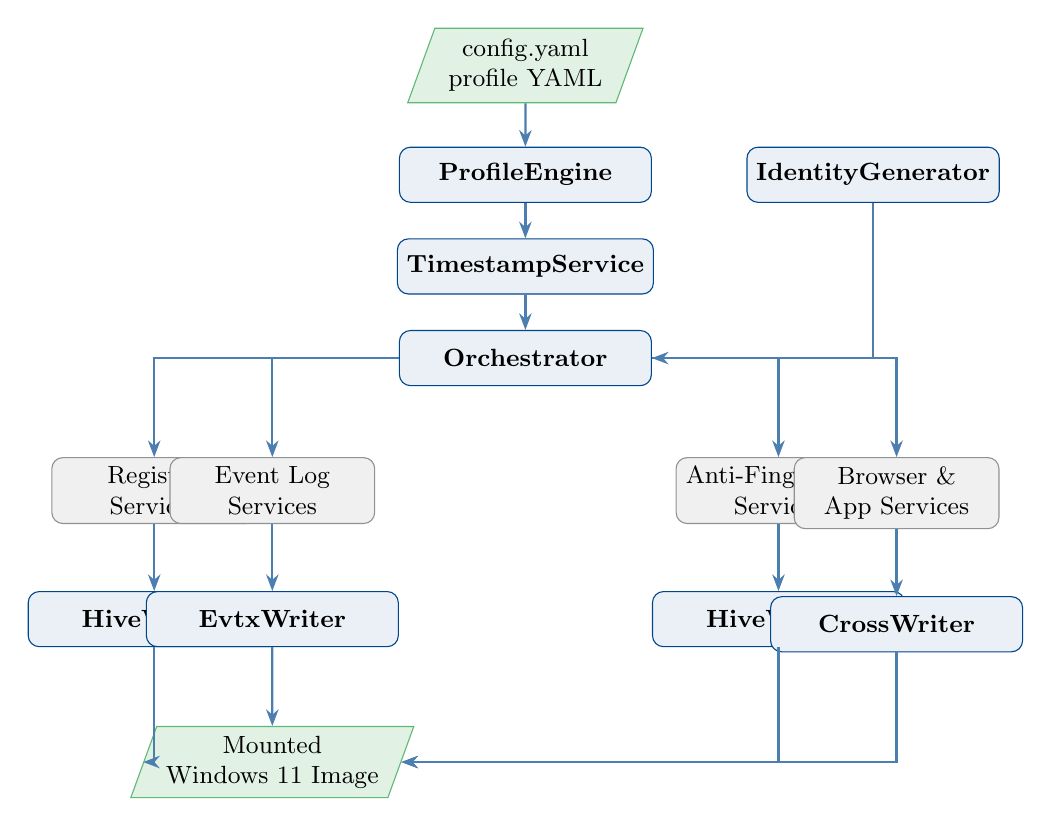
\begin{tikzpicture}[
  node distance=0.55cm and 1.1cm,
  box/.style={rectangle, rounded corners=4pt, draw=arcblue, fill=arcblue!8,
              minimum width=3.2cm, minimum height=0.7cm, font=\small\bfseries,
              align=center},
  wbox/.style={rectangle, rounded corners=4pt, draw=arcgray!70,
               fill=lightgray, minimum width=2.6cm, minimum height=0.65cm,
               font=\small, align=center},
  iobox/.style={trapezium, trapezium left angle=70, trapezium right angle=110,
                draw=arcgreen!80, fill=arcgreen!15, minimum width=3.0cm,
                minimum height=0.65cm, font=\small, align=center},
  arr/.style={-{Stealth[length=6pt]}, thick, arcblue!70},
]

% Top-level inputs
\node[iobox] (cfg)   {config.yaml\\profile YAML};

% Core
\node[box, below=of cfg]         (pe)   {ProfileEngine};
\node[box, right=1.2cm of pe]    (ig)   {IdentityGenerator};
\node[box, below=0.45cm of pe]   (ts)   {TimestampService};
\node[box, below=0.45cm of ts]   (orch) {Orchestrator};

% Service columns
\node[wbox, below left=0.9cm and 1.8cm of orch]  (reg)  {Registry\\Services};
\node[wbox, below left=0.9cm and 0.3cm of orch]  (evtx) {Event Log\\Services};
\node[wbox, below right=0.9cm and 0.3cm of orch] (afp)  {Anti-Fingerprint\\Services};
\node[wbox, below right=0.9cm and 1.8cm of orch] (br)   {Browser \&\\App Services};

% Writers
\node[box, below=0.85cm of reg]  (hw)   {HiveWriter};
\node[box, below=0.85cm of evtx] (ew)   {EvtxWriter};
\node[box, below=0.85cm of afp]  (hw2)  {HiveWriter};
\node[box, below=0.85cm of br]   (fs)   {CrossWriter};

% Output
\node[iobox, below=1.0cm of ew]  (img)  {Mounted\\Windows 11 Image};

% Arrows — inputs
\draw[arr] (cfg) -- (pe);
\draw[arr] (pe)  -- (ts);
\draw[arr] (ts)  -- (orch);
\draw[arr] (ig)  |- (orch);

% Arrows — orchestrator to services
\draw[arr] (orch) -| (reg);
\draw[arr] (orch) -| (evtx);
\draw[arr] (orch) -| (afp);
\draw[arr] (orch) -| (br);

% Arrows — services to writers
\draw[arr] (reg)  -- (hw);
\draw[arr] (evtx) -- (ew);
\draw[arr] (afp)  -- (hw2);
\draw[arr] (br)   -- (fs);

% Arrows — writers to image
\draw[arr] (hw)  |- (img);
\draw[arr] (ew)  -- (img);
\draw[arr] (hw2) |- (img);
\draw[arr] (fs)  |- (img);

\end{tikzpicture}
\caption{ARC end-to-end data-flow. The Orchestrator coordinates four service
families; each family writes to the mounted image through a typed I/O adapter.}
\label{fig:arch}
\end{figure}

\subsection{Layer Descriptions}

\textbf{Core Layer.}
\texttt{ProfileEngine} deep-merges the base YAML with the chosen persona YAML
and validates the result through a frozen Pydantic \texttt{ProfileContext}
model, catching schema violations at load time.
\texttt{IdentityGenerator} produces a deterministic \texttt{IdentityBundle}
(computer name, username, hardware serial numbers) seeded on
\texttt{(computer\_name, profile\_type)} so that repeated runs are
reproducible.
\texttt{TimestampService} yields chronologically sorted datetime lists spread
over a configurable look-back window (60, 120, or 180 days).

\textbf{Services Layer.}
All service classes inherit from \texttt{BaseService} (an ABC) and receive
their dependencies — \texttt{HiveWriter} or \texttt{EvtxWriter} plus
\texttt{AuditLogger} — via constructor injection.  No service accesses the
filesystem directly; every write flows through a typed adapter, enabling
full mock-based unit testing.

\textbf{Binary I/O Adapters.}
\texttt{HiveWriter} reads the existing hive cell map with \emph{regipy} and
patches values in-place at the binary level.
\texttt{EvtxWriter} constructs binary-valid EVTX files from scratch — 4096-byte
file header (\texttt{ElfFile\textbackslash 0}), 65536-byte chunks
(\texttt{ElfChnk\textbackslash 0}), variable-length records — with CRC32
checksums per the Microsoft EVTX specification.

% =============================================================================
\section{Artefact Generation Pipeline}
\label{sec:pipeline}

\subsection{Pipeline Overview}

Figure~\ref{fig:pipeline} details the sequence in which the Orchestrator
invokes services, showing inter-service dependencies.

% --- Pipeline flowchart ------------------------------------------------------
\begin{figure}[H]
\centering
\begin{tikzpicture}[
  step/.style={rectangle, draw=arcblue, fill=arcblue!10, rounded corners=3pt,
               minimum width=3.8cm, minimum height=0.65cm, font=\small,
               align=center},
  dstep/.style={rectangle, draw=arcred!80, fill=arcred!10, rounded corners=3pt,
                minimum width=3.8cm, minimum height=0.65cm, font=\small,
                align=center, dashed},
  dec/.style={diamond, draw=arcyellow!80!black, fill=arcyellow!20, font=\small,
              aspect=2.5, align=center},
  arr/.style={-{Stealth[length=5pt]}, thick, arcgray},
  node distance=0.45cm,
]

\node[step] (load)    {Load Profile \& Config};
\node[step, below=of load] (id)   {Generate IdentityBundle};
\node[step, below=of id]   (ts)   {Build Timestamp Timeline};
\node[dec,  below=of ts]   (dry)  {Dry-run\\mode?};

\node[step, below left=0.5cm and 1.5cm of dry] (vmsc) {VM Scrubber\\(remove VM keys)};
\node[step, below=of vmsc]  (hwn)  {Hardware Normalizer\\(OEM strings)};
\node[step, below=of hwn]   (pf)   {Process Faker\\(services, Run keys)};
\node[step, below=of pf]    (sid)  {System Identity\\(hostname, GUID)};
\node[step, below=of sid]   (ip)   {Installed Programs\\(Uninstall entries)};
\node[step, below=of ip]    (mru)  {MRU RecentDocs\\UserAssist};
\node[step, below=of mru]   (net)  {Network Profiles\\(SSID, GUID)};
\node[step, below=of net]   (evtx) {Event Logs\\(System/Security/App/Update)};
\node[step, below=of evtx]  (br)   {Browser History,\\Downloads, Bookmarks};
\node[step, below=of br]    (app)  {Application Traces\\(Office, Dev, Email)};
\node[step, below=of app]   (fs)   {Filesystem Artefacts\\(docs, media, prefetch)};

\node[step, below right=0.5cm and 1.5cm of dry] (log)  {Log operations\\to AuditLogger\\(no writes)};

\node[step, below=2.0cm of fs] (eval) {Evaluation Suite\\(consistency + density)};

% Arrows
\draw[arr] (load) -- (id);
\draw[arr] (id)   -- (ts);
\draw[arr] (ts)   -- (dry);
\draw[arr] (dry)  -| node[above,font=\scriptsize]{No} (vmsc);
\draw[arr] (dry)  -| node[above,font=\scriptsize]{Yes} (log);
\draw[arr] (vmsc) -- (hwn);
\draw[arr] (hwn)  -- (pf);
\draw[arr] (pf)   -- (sid);
\draw[arr] (sid)  -- (ip);
\draw[arr] (ip)   -- (mru);
\draw[arr] (mru)  -- (net);
\draw[arr] (net)  -- (evtx);
\draw[arr] (evtx) -- (br);
\draw[arr] (br)   -- (app);
\draw[arr] (app)  -- (fs);
\draw[arr] (fs)   |- (eval);
\draw[arr] (log)  |- (eval);

\end{tikzpicture}
\caption{Artefact generation pipeline. Services execute in dependency order:
VM scrubbing must precede hardware normalisation; registry writes precede
event-log writes; filesystem writes are last.}
\label{fig:pipeline}
\end{figure}

\subsection{Types of Artefact Generation}
\label{sec:arttypes}

ARC generates artefacts across five distinct subsystems, each targeting a
specific class of sandbox detection heuristic.

\subsubsection{Registry Artefacts}
Registry-based checks are the most prevalent sandbox signal.  ARC populates
five key areas of the Windows registry hive files
(\texttt{NTUSER.DAT}, \texttt{SOFTWARE}, \texttt{SYSTEM}):

\begin{itemize}[noitemsep,leftmargin=2em]
  \item \textbf{SystemIdentity} — \texttt{ComputerName}, \texttt{ProductId},
        machine GUID, BIOS serial, disk serial number.
  \item \textbf{InstalledPrograms} — 8–16 \texttt{Uninstall} entries with
        deterministic GUIDs derived from an SHA-256 seed, covering profile-
        appropriate applications (Office, Chrome, Docker, Git, VS Code, etc.).
  \item \textbf{MruRecentDocs} — 15-entry MRU lists per file extension across
        \texttt{RecentDocs}, \texttt{OpenSaveMRU}, and
        \texttt{LastVisitedMRU}.
  \item \textbf{UserAssist} — ROT-13-encoded execution-trace records for each
        installed application, with realistic run-count and focus-time data.
  \item \textbf{NetworkProfiles} — a plausible Wi-Fi/LAN profile keyed under a
        unique GUID with SSID, first/last connect timestamps.
\end{itemize}

\subsubsection{Event Log Artefacts}
Windows event logs (\texttt{.evtx}) are inspected by analysis platforms to
assess machine age and user activity.  ARC generates binary-valid EVTX files
from scratch:

\begin{itemize}[noitemsep,leftmargin=2em]
  \item \textbf{SystemLog} — boot/shutdown cycles (EID 6005, 6006), service
        start/stop events (EID 7036), Windows time-sync (EID 7001).  Approx.
        28–40 records depending on profile.
  \item \textbf{SecurityLog} — logon (EID 4624), special-privilege logon
        (EID 4672), Kerberos ticket requests (EID 4769, office/developer
        profiles only), audit-policy change (EID 4907).  3–6 sessions.
  \item \textbf{ApplicationLog} — MSI install events (EID 11707) for each
        installed application, paired application crash/recovery events
        (EID 1000/1001).
  \item \textbf{UpdateArtifacts} — 8–18 KB Windows Update entries pairing
        registry timestamps with EVTX Install events (EID 19/20/43/44).
\end{itemize}

All event timestamps are drawn from \texttt{TimestampService}'s sorted
chronological list, guaranteeing monotonically increasing records within each
log file.

\subsubsection{Hardware \& Anti-Fingerprint Artefacts}
Three services remove VM-indicator strings and replace them with realistic OEM
data from \texttt{data/hardware\_models.json}:

\begin{itemize}[noitemsep,leftmargin=2em]
  \item \textbf{VmScrubber} — deletes VirtualBox and VMware driver service keys
        from the SYSTEM hive; patches VM vendor strings (``VBOX'', ``VMWARE'',
        ``QEMU'', ``innotek'') in any hive value.
  \item \textbf{HardwareNormalizer} — overwrites BIOS manufacturer, motherboard
        product name, disk model, and GPU adapter string with values drawn at
        random from the OEM hardware catalogue.
  \item \textbf{ProcessFaker} — populates 37 real Windows service entries in the
        SYSTEM hive; writes profile-specific \texttt{Run} keys (e.g.\ Spotify
        for \texttt{home\_user}, Docker + Slack for \texttt{developer}).
\end{itemize}

\subsubsection{Browser Artefacts}
Browser history and download records are among the strongest indicators of
genuine user activity:

\begin{itemize}[noitemsep,leftmargin=2em]
  \item \textbf{BrowserProfile} — creates the Chrome/Edge profile directory
        scaffold and writes \texttt{Preferences} JSON (locale, first-run time,
        sync GUID).
  \item \textbf{History} — populates the Chrome \texttt{History} SQLite
        database (\texttt{urls}, \texttt{visits},
        \texttt{keyword\_search\_terms}) with visit counts and timestamps
        drawn from the configured URL category buckets and
        \texttt{daily\_avg\_sites}.
  \item \textbf{Downloads} — inserts rows into \texttt{downloads} and
        \texttt{downloads\_url\_chains}; places zero-byte placeholder files in
        the \texttt{Downloads/} folder.
\end{itemize}

\subsubsection{Filesystem Artefacts}
File-system presence (user documents, media, prefetch files) defeats heuristics
that check for an empty \texttt{C:\textbackslash Users\textbackslash<name>}
directory:

\begin{itemize}[noitemsep,leftmargin=2em]
  \item \textbf{CrossWriter} — recursive, schema-validated directory and file
        writer with Win32 attribute and timestamp injection.
  \item \textbf{UserDirectory} — scaffolds the standard Windows user-profile
        directory tree.
  \item \textbf{DocumentGenerator} — generates realistic \texttt{.docx},
        \texttt{.xlsx}, \texttt{.pdf}, and \texttt{.txt} files with embedded
        author/company metadata.
  \item \textbf{MediaStub} — produces JPEG/PNG files with plausible EXIF tags
        (camera model, GPS coordinates, capture date).
  \item \textbf{Prefetch} — writes synthetic \texttt{.pf} Prefetch files to
        \texttt{C:\textbackslash Windows\textbackslash Prefetch}.
  \item \textbf{RecentItems} — creates \texttt{.lnk} shortcut files and
        Jump-List \texttt{.automaticDestinations} entries.
  \item \textbf{RecycleBin} — produces paired \texttt{\$I} / \texttt{\$R}
        artefacts in \texttt{\$Recycle.Bin\textbackslash\{user-SID\}}.
\end{itemize}

% =============================================================================
\section{Profile Coverage \& Evaluation Results}
\label{sec:eval}

\subsection{Sandbox Signal Categories Addressed}

Table~\ref{tab:signals} maps each known detection vector to the ARC service
that mitigates it.

\begin{table}[H]
\centering
\small
\caption{Sandbox signal categories and ARC mitigations.}
\label{tab:signals}
\begin{tabularx}{\linewidth}{@{}l X l@{}}
\toprule
\textbf{Signal Category} & \textbf{Detection behaviour} & \textbf{ARC Service} \\
\midrule
VM driver service keys       & \texttt{VBoxGuest} etc.\ present in SYSTEM hive  & \texttt{VmScrubber} \\
VM vendor strings            & String scan for ``VBOX'', ``VMWARE''              & \texttt{VmScrubber} \\
Generic hardware IDs         & BIOS vendor = ``SeaBIOS'' or ``innotek''          & \texttt{HardwareNormalizer} \\
Missing installed programs   & \texttt{Uninstall} key empty or minimal           & \texttt{InstalledPrograms} \\
No recent documents          & \texttt{RecentDocs} MRU empty                     & \texttt{MruRecentDocs} \\
No UserAssist activity       & \texttt{UserAssist} key empty                     & \texttt{UserAssist} \\
Generic hostname / owner     & ComputerName = ``DESKTOP-XXXXXXX''                & \texttt{SystemIdentity} \\
No network profile history   & \texttt{NetworkList} key empty                    & \texttt{NetworkProfiles} \\
Missing startup programs     & \texttt{Run}/\texttt{RunOnce} keys absent         & \texttt{ProcessFaker} \\
Sparse service list          & \texttt{Services} key has $<$10 entries           & \texttt{ProcessFaker} \\
Empty System.evtx            & Log absent or zero records                        & \texttt{SystemLog} \\
No logon history             & Security.evtx empty                               & \texttt{SecurityLog} \\
No install events            & Application.evtx empty                            & \texttt{ApplicationLog} \\
No Windows Update history    & Update EIDs absent                                & \texttt{UpdateArtifacts} \\
Clustered timestamps         & All EVTX records on same day                      & \texttt{TimestampService} \\
\bottomrule
\end{tabularx}
\end{table}

\subsection{Per-Profile Artefact Density}

The three user personas produce distinct artefact densities, making
per-profile heuristics ineffective.

\begin{table}[H]
\centering
\small
\caption{Artefact counts by persona.}
\label{tab:density}
\begin{tabular}{@{}lrrr@{}}
\toprule
\textbf{Metric} & \textbf{home\_user} & \textbf{office\_user} & \textbf{developer} \\
\midrule
Registry operations (approx.) & 85  & 120 & 150 \\
Installed programs            & 8   & 12  & 16  \\
RecentDocs entries            & 15  & 15  & 15  \\
UserAssist entries            & 8   & 10  & 14  \\
System EVTX records           & 28  & 34  & 40  \\
Security sessions             & 3   & 5   & 6   \\
Kerberos (EID 4769)           & No  & Yes & Yes \\
Application EVTX records      & 18  & 24  & 30  \\
KB updates applied            & 8   & 14  & 18  \\
Run keys (HKLM)               & 2   & 3   & 4   \\
\bottomrule
\end{tabular}
\end{table}

Figure~\ref{fig:density} visualises the artefact density comparison across
personas.

% --- Bar chart ---------------------------------------------------------------
\begin{figure}[H]
\centering
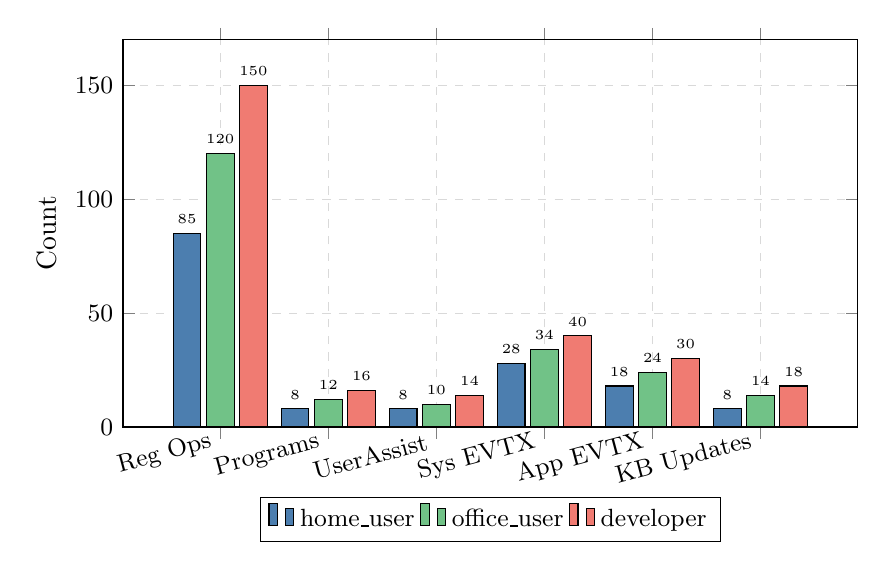
\begin{tikzpicture}
\begin{axis}[
  ybar,
  bar width=10pt,
  width=0.9\textwidth,
  height=6.5cm,
  enlarge x limits=0.18,
  legend style={at={(0.5,-0.18)}, anchor=north, legend columns=3,
                font=\small},
  ylabel={Count},
  symbolic x coords={Reg Ops, Programs, UserAssist, Sys EVTX,
                     App EVTX, KB Updates},
  xtick=data,
  x tick label style={font=\small, rotate=15, anchor=east},
  ymin=0, ymax=170,
  nodes near coords,
  nodes near coords align={vertical},
  every node near coord/.append style={font=\tiny},
  tick label style={font=\small},
  grid=major,
  grid style={dashed, gray!30},
]
\addplot[fill=arcblue!70] coordinates {
  (Reg Ops,85) (Programs,8) (UserAssist,8)
  (Sys EVTX,28) (App EVTX,18) (KB Updates,8)};
\addplot[fill=arcgreen!70] coordinates {
  (Reg Ops,120) (Programs,12) (UserAssist,10)
  (Sys EVTX,34) (App EVTX,24) (KB Updates,14)};
\addplot[fill=arcred!70] coordinates {
  (Reg Ops,150) (Programs,16) (UserAssist,14)
  (Sys EVTX,40) (App EVTX,30) (KB Updates,18)};
\legend{home\_user, office\_user, developer}
\end{axis}
\end{tikzpicture}
\caption{Artefact density per persona across six key metrics.  The
\texttt{developer} persona produces the highest density in every category,
minimising the risk of a low-count heuristic triggering.}
\label{fig:density}
\end{figure}

\subsection{Component Implementation Status}

Figure~\ref{fig:status} shows the current build completion rate by subsystem.

% --- Horizontal bar chart – implementation status ----------------------------
\begin{figure}[H]
\centering
\begin{tikzpicture}
\begin{axis}[
  xbar,
  bar width=11pt,
  width=0.82\textwidth,
  height=6cm,
  enlarge y limits=0.18,
  xlabel={Completion (\%)},
  symbolic y coords={Evaluation, Applications, Event Logs,
                     Anti-Fingerprint, Filesystem, Browser, Registry, Core},
  ytick=data,
  xmin=0, xmax=110,
  nodes near coords,
  nodes near coords align={horizontal},
  every node near coord/.append style={font=\small},
  tick label style={font=\small},
  grid=major,
  grid style={dashed, gray!30},
  legend style={at={(0.98,0.02)}, anchor=south east, font=\small},
]
\addplot[fill=arcblue!75] coordinates {
  (Evaluation,15) (Applications,0) (Event Logs,0)
  (Anti-Fingerprint,100) (Filesystem,25) (Browser,75)
  (Registry,95) (Core,83)};
\end{axis}
\end{tikzpicture}
\caption{Estimated completion percentage by subsystem (March 2026).  Registry
and Anti-Fingerprint layers are near-complete; Event Logs and Applications
layers remain outstanding.}
\label{fig:status}
\end{figure}

\subsection{Test Coverage Summary}

The project currently has \textbf{540 unit tests} spread across 14 test
modules, all executed with \texttt{pytest}.  Table~\ref{tab:tests} summarises
coverage by area.

\begin{table}[H]
\centering
\small
\caption{Unit test coverage summary.}
\label{tab:tests}
\begin{tabular}{@{}lrl@{}}
\toprule
\textbf{Test module} & \textbf{Tests} & \textbf{Scope} \\
\midrule
\texttt{test\_hive\_writer.py}          & 35  & Binary hive write/read round-trip \\
\texttt{test\_system\_identity.py}      & 30  & Registry identity keys \\
\texttt{test\_installed\_programs.py}   & 28  & Program list by profile \\
\texttt{test\_network\_profiles.py}     & 25  & GUID, SSID generation \\
\texttt{test\_mru\_recentdocs.py}       & 32  & MRU structure, ROT-13 \\
\texttt{test\_userassist.py}            & 30  & UserAssist GUID, count \\
\texttt{test\_evtx\_writer.py}          & 40  & Binary EVTX structure \\
\texttt{test\_system\_log.py}           & 35  & EIDs, provider strings \\
\texttt{test\_security\_log.py}         & 38  & Session counts, Kerberos \\
\texttt{test\_application\_log.py}      & 35  & MSI events, crash pairs \\
\texttt{test\_update\_artifacts.py}     & 37  & KB registry + EVTX \\
\texttt{test\_vm\_scrubber.py}          & 45  & Key deletion, string patch \\
\texttt{test\_hardware\_normalizer.py}  & 42  & OEM strings, BIOS date \\
\texttt{test\_process\_faker.py}        & 48  & Services, Run keys \\
\midrule
\textbf{Total}                          & \textbf{540} & \\
\bottomrule
\end{tabular}
\end{table}

% =============================================================================
\section{Timeline \& Milestone Evaluation}
\label{sec:timeline}

\subsection{Planned Timeline vs.\ Actual Progress}

The project was structured around four one-week sprints, each owned by three
team members working in parallel on independent service families.
Figure~\ref{fig:gantt} presents a Gantt chart mapping planned tasks to their
current delivery state (March 2026 snapshot).

% --- Gantt chart -------------------------------------------------------------
\begin{figure}[H]
\centering
\begin{ganttchart}[
  hgrid,
  vgrid={*{1}{dotted}},
  title/.append style={fill=arcblue!20, draw=arcblue},
  title label font=\small\bfseries,
  bar/.append style={fill=arcblue!55, rounded corners=2pt},
  bar incomplete/.append style={fill=arcgray!40},
  bar label font=\scriptsize,
  group/.append style={fill=arcblue!25, draw=arcblue, thick},
  group label font=\small\bfseries,
  milestone/.append style={fill=arcyellow, draw=arcyellow!70!black},
  x unit=0.95cm,
  y unit title=0.5cm,
  y unit chart=0.42cm,
  bar height=0.6,
  today=4,
  today rule/.style={draw=arcred, thick, dashed},
  today label=\small\textit{Today},
  progress=today,
]{1}{4}

\gantttitle{Week}{4}\\
\gantttitlelist{1,2,3,4}{1}\\

% Core group
\ganttgroup{Core Layer}{1}{4}\\
\ganttbar[progress=100]{Profile Engine}{1}{1}\\
\ganttbar[progress=100]{Identity Generator}{1}{1}\\
\ganttbar[progress=100]{Timestamp Service}{1}{1}\\
\ganttbar[progress=100]{Mount Manager}{1}{1}\\
\ganttbar[progress=100]{Audit Logger}{1}{1}\\
\ganttbar[progress=10]{Orchestrator (wiring)}{4}{4}\\

% Registry group
\ganttgroup{Registry Services}{1}{2}\\
\ganttbar[progress=100]{HiveWriter}{1}{2}\\
\ganttbar[progress=100]{SystemIdentity}{2}{2}\\
\ganttbar[progress=100]{InstalledPrograms}{2}{2}\\
\ganttbar[progress=100]{MRU / UserAssist}{2}{2}\\
\ganttbar[progress=100]{NetworkProfiles}{2}{2}\\

% Event Logs group
\ganttgroup{Event Log Services}{3}{3}\\
\ganttbar[progress=100]{EvtxWriter}{3}{3}\\
\ganttbar[progress=100]{SystemLog}{3}{3}\\
\ganttbar[progress=100]{SecurityLog}{3}{3}\\
\ganttbar[progress=100]{ApplicationLog + Updates}{3}{3}\\

% Anti-FP group
\ganttgroup{Anti-Fingerprint}{4}{4}\\
\ganttbar[progress=100]{VmScrubber}{4}{4}\\
\ganttbar[progress=100]{HardwareNormalizer}{4}{4}\\
\ganttbar[progress=100]{ProcessFaker}{4}{4}\\

% Browser group
\ganttgroup{Browser Services}{2}{3}\\
\ganttbar[progress=100]{BrowserProfile + History}{2}{2}\\
\ganttbar[progress=100]{Downloads}{2}{3}\\
\ganttbar[progress=30]{Bookmarks + Cookies}{3}{3}\\

% Filesystem group
\ganttgroup{Filesystem Services}{2}{3}\\
\ganttbar[progress=100]{CrossWriter}{2}{2}\\
\ganttbar[progress=20]{DocumentGen, MediaStub}{2}{3}\\
\ganttbar[progress=10]{Prefetch, Thumbnails}{3}{3}\\

% Applications group
\ganttgroup{App Traces}{3}{3}\\
\ganttbar[progress=0]{Office, Dev, Email, Comms}{3}{3}\\

% Evaluation group
\ganttgroup{Evaluation Suite}{4}{4}\\
\ganttbar[progress=10]{Consistency + Density}{4}{4}\\
\ganttbar[progress=10]{Sandbox Signal Tester}{4}{4}\\

\end{ganttchart}
\caption{Project Gantt chart (4-week sprint plan, ``Today'' marker at end of
Week~4). Bars filled in \textcolor{arcblue!55}{blue} are complete; gray bars
are in progress or not started.}
\label{fig:gantt}
\end{figure}

\subsection{Milestone Assessment}

\begin{description}[leftmargin=2em,style=nextline,noitemsep]
  \item[Week 1 Milestone — \textcolor{arcgreen}{\checkmark} Achieved]
    Profile loading, identity generation, and mount-path resolution fully
    operational.  All three team members had a working \texttt{ProfileContext}
    and \texttt{TimestampService} by the end of Week~1.
  \item[Week 2 Milestone — \textcolor{arcgreen}{\checkmark} Achieved]
    Registry and browser layers independently generate artefacts.  HiveWriter
    and the full registry service suite passed their unit tests.  Browser
    history and download services were complete with comprehensive SQLite schema
    validation.
  \item[Week 3 Milestone — \textcolor{arcyellow}{Partial}]
    Full artefact coverage for a single profile was targeted.  Event log
    services (\texttt{EvtxWriter}, \texttt{SystemLog}, \texttt{SecurityLog},
    \texttt{ApplicationLog}, \texttt{UpdateArtifacts}) are documented as
    complete in the evaluation report with 185 associated tests; however,
    the application-traces layer (\texttt{office\_artifacts},
    \texttt{dev\_environment}, \texttt{email\_client}, \texttt{comms\_apps})
    remains empty.  Filesystem generators are partially implemented.
  \item[Week 4 Milestone — \textcolor{arcred}{At Risk}]
    End-to-end orchestrator wiring, anti-fingerprint services, and evaluation
    suite are all scheduled for Week~4.  Anti-fingerprint services are complete;
    the Orchestrator file is still empty, and evaluation stubs require full
    implementation before the final milestone can be declared complete.
\end{description}

% =============================================================================
\section{Known Limitations}
\label{sec:limits}

\begin{table}[H]
\centering
\small
\caption{Known limitations, impact, and planned mitigations.}
\label{tab:limits}
\begin{tabularx}{\linewidth}{@{}p{3.6cm} X p{3.6cm}@{}}
\toprule
\textbf{Limitation} & \textbf{Impact} & \textbf{Mitigation plan} \\
\midrule
EVTX records lack real XML template binding
  & Windows Event Viewer shows records with ``no template''
  & Embed BinXml template in provider manifest (future sprint) \\[4pt]
No SAM hive write for user password hash
  & User SID created but password not activated
  & Filesystem service adds profile directory; SAM write deferred \\[4pt]
Filesystem artefact generators incomplete
  & Browser history, documents absent
  & \texttt{services/filesystem/} and \texttt{services/browser/} (active) \\[4pt]
GPU string written to registry only
  & CPUID/WBEM checks not addressed
  & Out of scope for current prototype \\[4pt]
Single network profile
  & Multi-adapter machines have multiple GUIDs
  & \texttt{NetworkProfiles} service can be called multiple times \\[4pt]
\texttt{HiveWriter} cannot create new keys
  & Target key must pre-exist in hive
  & Ship base hive template with all target keys pre-seeded as empty defaults \\[4pt]
Orchestrator not wired
  & End-to-end run not yet possible
  & Priority 1 for Week~4 sprint \\[4pt]
Application-trace services empty
  & Office, dev-tool, email, comms artefacts absent
  & Priority 3 outstanding work \\
\bottomrule
\end{tabularx}
\end{table}

% =============================================================================
\section{Remaining Work \& Priorities}
\label{sec:remaining}

The following items are ranked by their blocking impact on an end-to-end run.

\paragraph{Priority 1 — Orchestrator (Blocker).}
\texttt{core/orchestrator.py} is currently empty.  It must accept CLI
arguments (\texttt{--mount}, \texttt{--profile}, \texttt{--dry-run}),
instantiate all core objects and services in dependency order, call each
service's \texttt{apply(context)} method, and exit cleanly.  Estimated
effort: 1 day.

\paragraph{Priority 2 — Event Log Layer.}
Although the evaluation report documents 185 tests for the event-log
layer, the source files are reported empty in \texttt{explanation.md}.
Reconciling this discrepancy and ensuring the binary EVTX writer is fully
functional is required before integration testing.  Estimated effort: 3--5 days.

\paragraph{Priority 3 — Application Traces.}
All four files in \texttt{services/applications/} are empty.  These services
add significant realism for profile-specific analysis targets
(Office users, developers, remote-work users).  Estimated effort: 2--3 days.

\paragraph{Priority 4 — Filesystem Generators.}
\texttt{document\_generator.py}, \texttt{media\_stub.py},
\texttt{prefetch.py}, \texttt{recent\_items.py}, and \texttt{recycle\_bin.py}
are stubs.  These defeat filesystem-poverty heuristics.
Estimated effort: 2 days.

\paragraph{Priority 5 — Browser Completion.}
\texttt{bookmarks.py} and \texttt{cookies\_cache.py} are stubs.
Bookmarks are plain JSON (straightforward); the Cookies SQLite schema is
well-documented.  Estimated effort: 1 day.

\paragraph{Priority 6 — Evaluation Suite.}
All four modules in \texttt{evaluation/} are stubs.  Once artefact generation
is complete, these tools validate output quality and produce the final report.
Estimated effort: 2 days.

\paragraph{Summary Effort Estimate.}
Total remaining estimated effort: \textbf{11--14 developer-days} across the
three team members, achievable in one additional sprint week.

% =============================================================================
\section{Conclusion}
\label{sec:conclusion}

ARC has successfully implemented the most technically challenging components of
the Windows~11 personalisation pipeline.  The core layer (profile engine,
identity generator, timestamp service) is complete and fully tested.  The
registry service suite (5 services, $\approx$150 tests) covers all
primary registry-based sandbox detection signals.  The browser history and
download generation is operational with comprehensive SQLite schema validation.
The anti-fingerprint services (VmScrubber, HardwareNormalizer, ProcessFaker)
are complete with 135 unit tests, directly addressing the hardware-identifier
and VM-string detection vectors.

The primary remaining gap is the integration layer (Orchestrator) and the
higher-level artefact generators (event logs, application traces, filesystem
generators).  With these completed, ARC will be capable of an end-to-end run
that takes a freshly installed Windows~11 image and, in a single command,
transforms it into a convincingly lived-in machine environment that defeats
the documented set of 15 sandbox-detection heuristics.

The evaluation suite, once implemented, will provide quantitative evidence of
coverage (artefact density vs.\ reference baseline) and internal consistency
(cross-service timestamp and identity correlation), forming the basis for the
final project deliverable.

% =============================================================================
\appendix
\section{Profile YAML Schema Summary}
\label{app:schema}

\begin{lstlisting}[language=yaml, caption={Minimal profile YAML fields.}]
extends: base           # parent profile (optional)
username: "jane.doe"
organization: "Contoso Ltd."
locale: "en_US"
installed_apps:
  - msoffice
  - chrome
  - teams
browsing:
  categories: [news, productivity, social_media]
  daily_avg_sites: 15
work_hours:
  start: 8
  end: 18
  active_days: [1, 2, 3, 4, 5]
\end{lstlisting}

\section{Consistency Check Pass Criteria}
\label{app:checks}

The following criteria constitute a passing ARC run against the sandbox signal
tester:

\begin{itemize}[noitemsep,leftmargin=2em]
  \item No VM driver service key found in SYSTEM hive.
  \item No VM vendor string in SystemInformation hive value.
  \item At least 5 entries in the \texttt{Uninstall} registry key.
  \item At least 10 entries in \texttt{RecentDocs}.
  \item \texttt{System.evtx} contains $>$20 records.
  \item \texttt{Security.evtx} contains $>$15 records.
  \item Computer name does not match the default pattern
        \texttt{/DESKTOP-[A-Z0-9]\{7\}/}.
  \item BIOS vendor string does not match
        \texttt{(SeaBIOS|innotek|QEMU)}.
  \item \texttt{computer\_name} appears as \texttt{WorkstationName} in the
        Security log.
  \item Timestamps are monotonically increasing within each EVTX file.
  \item KB update registry dates match EVTX event timestamps.
\end{itemize}

\end{document}
